\chapter{\ehtxt{Numerical} schemes for computing extracellular potentials}
\label{sec:LFPy}
\ghnote{Torbjorn/Espen will write most this.}
\ghnote{La inn forslag til intro her:}

%%%%%%%%%%%%%%%%%%%%%%%%%%%%%%%%%%%%%%%%%%%%%

The \ehtxt{established \sout{standard}} way of computing extracellular potentials is to use a two-step multicompartment + volume conduction (MC+VC) scheme,
which can be summarized as:

\begin{itemize}
\item {\bf Step 1:} Compute the electrical activity of neurons using a the multicompartment (MC) framework presented in \Fref{chap:Neuron}, assuming that it is unaffected by whatever goes on in the extracellular space.
\item {\bf Step 2:} Compute the extracellular potential $\phi$ resulting from the neural transmembrane currents computed in step 1, using Volume Conductor (VC) theory (Chapters \Fref{chap:VC}-\ref{chap:Sigma}). 
\end{itemize}

The MC+VC scheme is not self-consistent, since Step 1 computes the neurodynamics under the assumption that $\phi$ is \ehtxt{unaffected by transmembrane currents \sout{zero (grounded extracellular space)}},
and Step 2 uses this neurodynamics to compute a non-zero extracellular potential.
\ehnote{I wonder if we should elaborate more on pt. 1: It is entirely possible to impose potentials different from zero and time varying with the current scheme and simultaneously estimate transmembrane currents. The main problem is that cable theory is 1D while real neurons are 3D (with the exception of structures such as axonal tracts).
Self-ephaptic effects should be entirely possible to account for using standard methods (NEURON) for cable models with 1D geometry (at least that's what I think!).}
There exist more complete and consistent schemes that account for both the ephaptic effects from $\phi$ on neurodynamics as well as for effects of ion concentration dynamics on neuronal activity of extracelluar potentials. In general, these more complete schemes require numerical simulations of both the neural and extracellular dynamics using finite element or finite difference methods, and are very computationally expensive.

In most scenarios, ephaptic effects from extracellular potentials on neurodynamics are small, and ion concentrations tend to stay close to baseline. When this is true, the simplifying approximations applied in the two-step scheme do not critically affect the accuracy of its predictions. As the MC+VC scheme is far more computationally efficient than any of the more complete schemes, it remains the gold standard for computing $\phi$ in large population models of neurons mimicking physiologically realistic scenarios. Also, designated software has been developed that makes it easy to perform simulations using the two-step-procedure. Therefore, the simulations in the application part of this book (Part 2) will predominantly be based on on the MC+VC-framework.

When aiming to make realistic simulations of extracellular potentials, one might need to simulate large networks containing thousands of neurons. This is computationally demanding, even on an efficient scheme like MC+VC.
\ehnote{Computational demands are linearly dependent on the total number of compartments, so this a "simple" problem to solve, just scale up your computer capability accordingly.}
As we showed in \Fref{chap:VC},
VC theory gave us \ehtxt{linear} analytical expression\ehtxt{s} for $\phi$ as a direct function of the neural current sources (Step 2), meaning that it is \ehtxt{usually} the simulations of the neurodynamics (Step 1) which is the bottleneck in the simulation. Below, we present computational schemes for the standard MC+VC approach, based on multicompartment neural models (Section \ref{sec:Schemes:LFPy}), and follow up with two strategies that may be applied to reduce the computational cost when computing the neurodynamics (Sections \ref{sec:Schemes:HybridLFPy}-\ref{sec:Schemes:KernelLFPy}). We end the chapter with a brief introduction of an alternative, and self-consistent framework (Section \ref{sec:VC:EMI}).

\ehnote{For meg gir det mer mening og organisere dette i reduksjonistisk rekkefoelge: (1) self-consistent; (2) MC+VC; (3) point-neuron spiking + MC + VC; (4) firing-rate + MC + VC.
Men uansett, burde ikke dette vaere del av "Applications"-kapitlet? Punkt 3 og 4 endrer i prinsippet ingenting med MV+VC formalismen - man disassosierer bare simulering av nettverksaktivitet (korrelasjoner) fra (MC+VC)-formalismen.}



%%%%%%

\section{\ehnote{}\ehtxt{Forward-model predictions from multicompartment neuron models}}
\label{sec:Schemes:LFPy}
\index{Multicompartment models}


Most models aiming to mimic the dynamics of a particular neuron or neural system except the simplest ball and stick like models are too complex to be solved analytically (cf. \Fref{chap:Neuron}).
Thus the set of partial differential equations (PDEs) and initial conditions representing voltage- and concentration-dependent ion channels, synapses, plasticity, neuronal geometry etc. of the full model will have to be solved numerically on computers.
The numerical solution of geometrically detailed cable models entails a discretization of the geometry into multiple compartments (hence MC) wherein the states of variables and their derivatives are estimated on a temporal grid which may be fixed or irregular.
While one could utilize general-purpose numerical solvers in order to compute resulting voltage fluctuations, transmembrane currents or axial currents,
a more feasible approach is utilization of one of several different software tools tailored for this purpose that have been developed in the past.
Such software greatly simplify the process of specifying the phenomenological or biophysically detailed model and choosing the appropriate numerical schemes for solving the resulting set of PDEs.
Such tools will also by default usually account for one of the main assumptions of standard cable theory, that is,
the spatial variation in membrane voltage across the entire morphology can be computed independently of any effect
transmembrane currents may have on the extracellular potential immediately outside the compartments (see chapter \Fref{chap:Neuron} for details).


The NEURON simulation environment\footnote{\href{https://neuron.yale.edu}{https://neuron.yale.edu}} \cite**{Hines1997} presently remains a prevalent choice for empiric-based simulations of MC neuron models as it supports both Windows-,
linux- and unix-based operating systems including MacOS,
and can be used with a GUI or in a programmatic fashion on laptops, desktop computers and in parallel on large-scale high-performance computing (HPC) facilities.
NEURON is also utilized as a simulator backend for other higher-level software such as
PyNN\footnote{\href{https://neuralensemble.org/PyNN/}{https://neuralensemble.org/PyNN/}} \cite**{Davison2008},
NetPyne\footnote{\href{http://www.netpyne.org}{http://www.netpyne.org}} \cite**{Dura_Bernal_2019},
BMTK\footnote{\href{https://alleninstitute.github.io/bmtk/}{https://alleninstitute.github.io/bmtk/}} \cite**{Dai2020},
LFPy\footnote{\href{https://lfpy.readthedocs.io}{https://lfpy.readthedocs.io}} \cite**{Linden2014,Hagen2018} etc.
Alternatives to NEURON with partially overlapping feature sets have been developed in the past in form of
MOOSE\footnote{\href{https://moose.ncbs.res.in}{https://moose.ncbs.res.in}} \cite**{Bhalla2008} and
GENESIS\footnote{\href{http://genesis-sim.org}{http://genesis-sim.org}} \cite**{Bower1998},
while software tailored for point-like neuron models such as
Brian\footnote{\href{https://briansimulator.org/}{https://briansimulator.org/}} \cite**{Stimberg2019} recently received support for biophysically detailed MC neuron models.
Another effort receiving funding from the EU Human Brain Project,
named Arbor\footnote{\href{https://arbor.readthedocs.io}{https://arbor.readthedocs.io}} \cite**{Akar2019},
aims to develop MC neuron simulation software from the ground up in order to fully exploit modern high-performance libraries and next generation hardware in the form of graphical processing units (GPUs) and massively parallel HPC facilities.


\subsubsection{Predicting axial and transmembrane currents}
\label{chap:LFPy_Ia_Im}

Here we will refrain from going into details on the inner workings of the above software tools,
but reiterate that both axial currents and transmembrane currents can be estimated if the set of PDEs can be solved numerically for the membrane voltage of the MC neuron model(s).
The membrane voltages of MC neuron models are typically assumed to be `measured' at the center of each compartment.
The axial and transmembrane currents of a non-branching piece of cable is given in continuous form by
%
\begin{eqnarray}
I_\mathrm{a}(x,t) &=& - \frac{1}{r_\mathrm{i}} \frac{\partial V_\mathrm{m}(x, t)}{\partial x} \text{~and} \\
i_\mathrm{m}(x, t) &=& - \frac{\partial I_\mathrm{a} (x, t)}{\partial x} = \frac{1}{r_\mathrm{i}} \frac{\partial^2 V_\mathrm{m}(x,t)}{\partial x^2}~,
\label{eq:LFPy_ia_im_continuous}
\end{eqnarray}
%
where the intracellular resistance per unit length $r_\mathrm{i}=4R_\mathrm{a}/\pi d^2$ can be given with unit \si{\ohm/\metre}.
Here, $R_\mathrm{a}$  and $d$ is the axial resistivity (\si{\ohm\metre}) and diameter (\si{\metre}) of the dendritic cable model, respectively (cf. \Fref{chap:Neuron}).
The unit for axial currents $I_\mathrm{a}(x, t)$ is \si{\ampere},
while the transmembrane current is per unit length (\si{\ampere/\metre}).
The location $x$ denotes the position along the piece of cable in one dimension (the cable equation is by definition 1D even if the different parts of a neuron may be assigned locations in 3D space).

For spatially discretized cable models the axial currents can be estimated per-compartment by the central difference approximation as
%
\begin{eqnarray}
I_\mathrm{a}(x_j, t) &\overset{h>0}{\approx}& - \frac{1}{r_\mathrm{i}} \frac{V_\mathrm{m}(x_j+\frac{h}{2}, t) - V_\mathrm{m}(x_j-\frac{h}{2}, t)}{h} \nonumber \\
		  &\overset{L_j=h}{=}& - \frac{\pi d_j^2}{4 R_\mathrm{a}} \frac{V(x_j - \frac{L_j}{2}, t) - V_\mathrm{m}(x + \frac{L_j}{2}, t)}{L_j} ~.
\label{eq:LFPy_ia_discrete}
\end{eqnarray}
%
Here, $x_j$ denotes midpoint location,
and the discretization constant $h$ is set equal to the compartment length $L_j$.
Its diameter is typically assumed to be constant,
and the cylindrical compartment is a straight along its length axis.
\ehnote{True for NEURON, but not for Arbor which adapts a FDM type scheme in 1D corresponding to electric compartments made up by series of conical frusta.}
Note that it is possible to swap the central difference approximation
by the forward and  backward difference approximation estimating axial currents for each half-compartment respectively as in \cite**{Hagen2018},
but we will not go into further detail here.

We next outline how the membrane potential can be estimated at the end points of each compartment $x \in \{x_j-L_j/2, x_j+L_j/2\}$,
which may connected to none, one or several other end points of other compartments,
when the neural simulation software returns the midpoint potential $V_\mathrm{m}(x_j, t)$ for every $j \in \{1, \cdots, N \}$ compartment.
For terminating compartments (i.e., one or both ends has no connecting compartments and sealed ends) we may define
%
\begin{eqnarray}
V_\mathrm{m}(x_j - L_j/2, t) &\equiv& V_\mathrm{m}(x_j, t)~\mathrm{and/or} \nonumber \\
V_\mathrm{m}(x_j + L_j/2, t) &\equiv& V_\mathrm{m}(x_j, t)~, \nonumber
\end{eqnarray}
%
depending on which end(s) has no electric connections.
(This step effectively utilize the forward/backward difference approximation to first derivatives but only to terminating compartments.
If both ends terminate, the axial current will be zero as the voltage is implicitly assumed to be iso-potential along the compartment axis.)

For a number $N$ child compartments connected at the end point location $(x_j+L_j/2)$ of the parent compartment (\Fref{fig:LFPy_circuits}C) the potential can be computed from the parent- and child-compartment mid-point potentials as \cite**{Hagen2018}

\begin{equation}
V_\mathrm{m}(x_j+L_j/2, t) = \frac{\sum_{n=0}^N V_\mathrm{m}(x_{j+n}, t) / R_{j+n}}{\sum_{n=0}^N 1 / R_{j+n}}~,
\label{eq:LFPy_V_connect_point}
\end{equation}
%
where the connecting node to mid point resistances
%
\begin{eqnarray}
R_{j+n} &=& \frac{2 R_\mathrm{a}L_{j+n}}{\pi d_{j+n}^2} ~.
\end{eqnarray}

For child compartments connecting to the mid point of the parent compartment,
the corresponding potential at the branch point seen by any number of child segments is per definition the same as the mid point potential of the parent, that is,
\begin{equation}
V_\mathrm{m}(x_{j+n}-L_{j+n} / 2, t) \equiv V_\mathrm{m}(x_j, t) ~.
\end{equation}

Up to this point, we have provided the basic `machinery' needed in order to compute the discrete axial currents in a MC neuron model,
independently of specific and non-specific ion-channel currents, synaptic currents, capacitive currents etc. which may be present in the membrane of biophysically detailed MC neuron models.
By our application of the central difference approximation to the first derivative,
it is in these derivations then implicitly assumed that the axial current is approximately constant along the entire length of the compartment,
which in turn imply that the the membrane voltage varies approximately linearly with position.
The naive computational neuroscientist should remind her/himself that this assumption is likely to be violated if the spatial discretization chosen for the model neuron(s) is too coarse.
%
Also the transmembrane currents may be estimated on a per-compartment basis in a similar manner using the central difference approximation to the 2nd derivative as
%
\begin{eqnarray}
i_\mathrm{m}(x_j, t) &\overset{h>0}{\approx}& \frac{1}{r_\mathrm{i}} \frac{V_\mathrm{m}(x_j + \frac{h}{2}, t) - V_\mathrm{m}(x_j, t)+ V_\mathrm{m}(x_j - \frac{h}{2}, t)}{h^2 / 4} \nonumber \\
		&\overset{L_j=h}{=}& \frac{\pi d_j^2}{R_\mathrm{a}} \frac{V_\mathrm{m}(x_j + \frac{L_j}{2}, t) - V_\mathrm{m}(x_j, t) + V_\mathrm{m}(x_j - \frac{L_j}{2}, t)}{L_j^2} ~.
\label{eq:LFPy_im_discrete}
\end{eqnarray}


This machinery may appear as a bit of a hurdle to implement for the purpose of computing extracellular potentials or magnetic signals,
but thankfully MC neuron modeling software such as NEURON and Arbor provides native support for computing the transmembrane current (\si{\ampere}) and/or transmembrane current density per surface membrane area (\si{\ampere/\metre^2}) for each compartment.
Dependent on the implementation in the neural simulation software,
a more direct measure of the transmembrane currents is indeed computing the sum over all capacitive currents, specific and non-specific ion-channel currents, synapse currents etc. (cf. \Fref{chap:Neuron}).
%
The current state is however a bit more dire with regards to predicting axial current per compartment (or half-compartment \cite**{Hagen2018}).
For now, we will emphasize that typical extracellular measures of extracellular electric or even magnetic signals can be derived from the transmembrane currents alone.

\begin{figure}[!ht]
\begin{center}
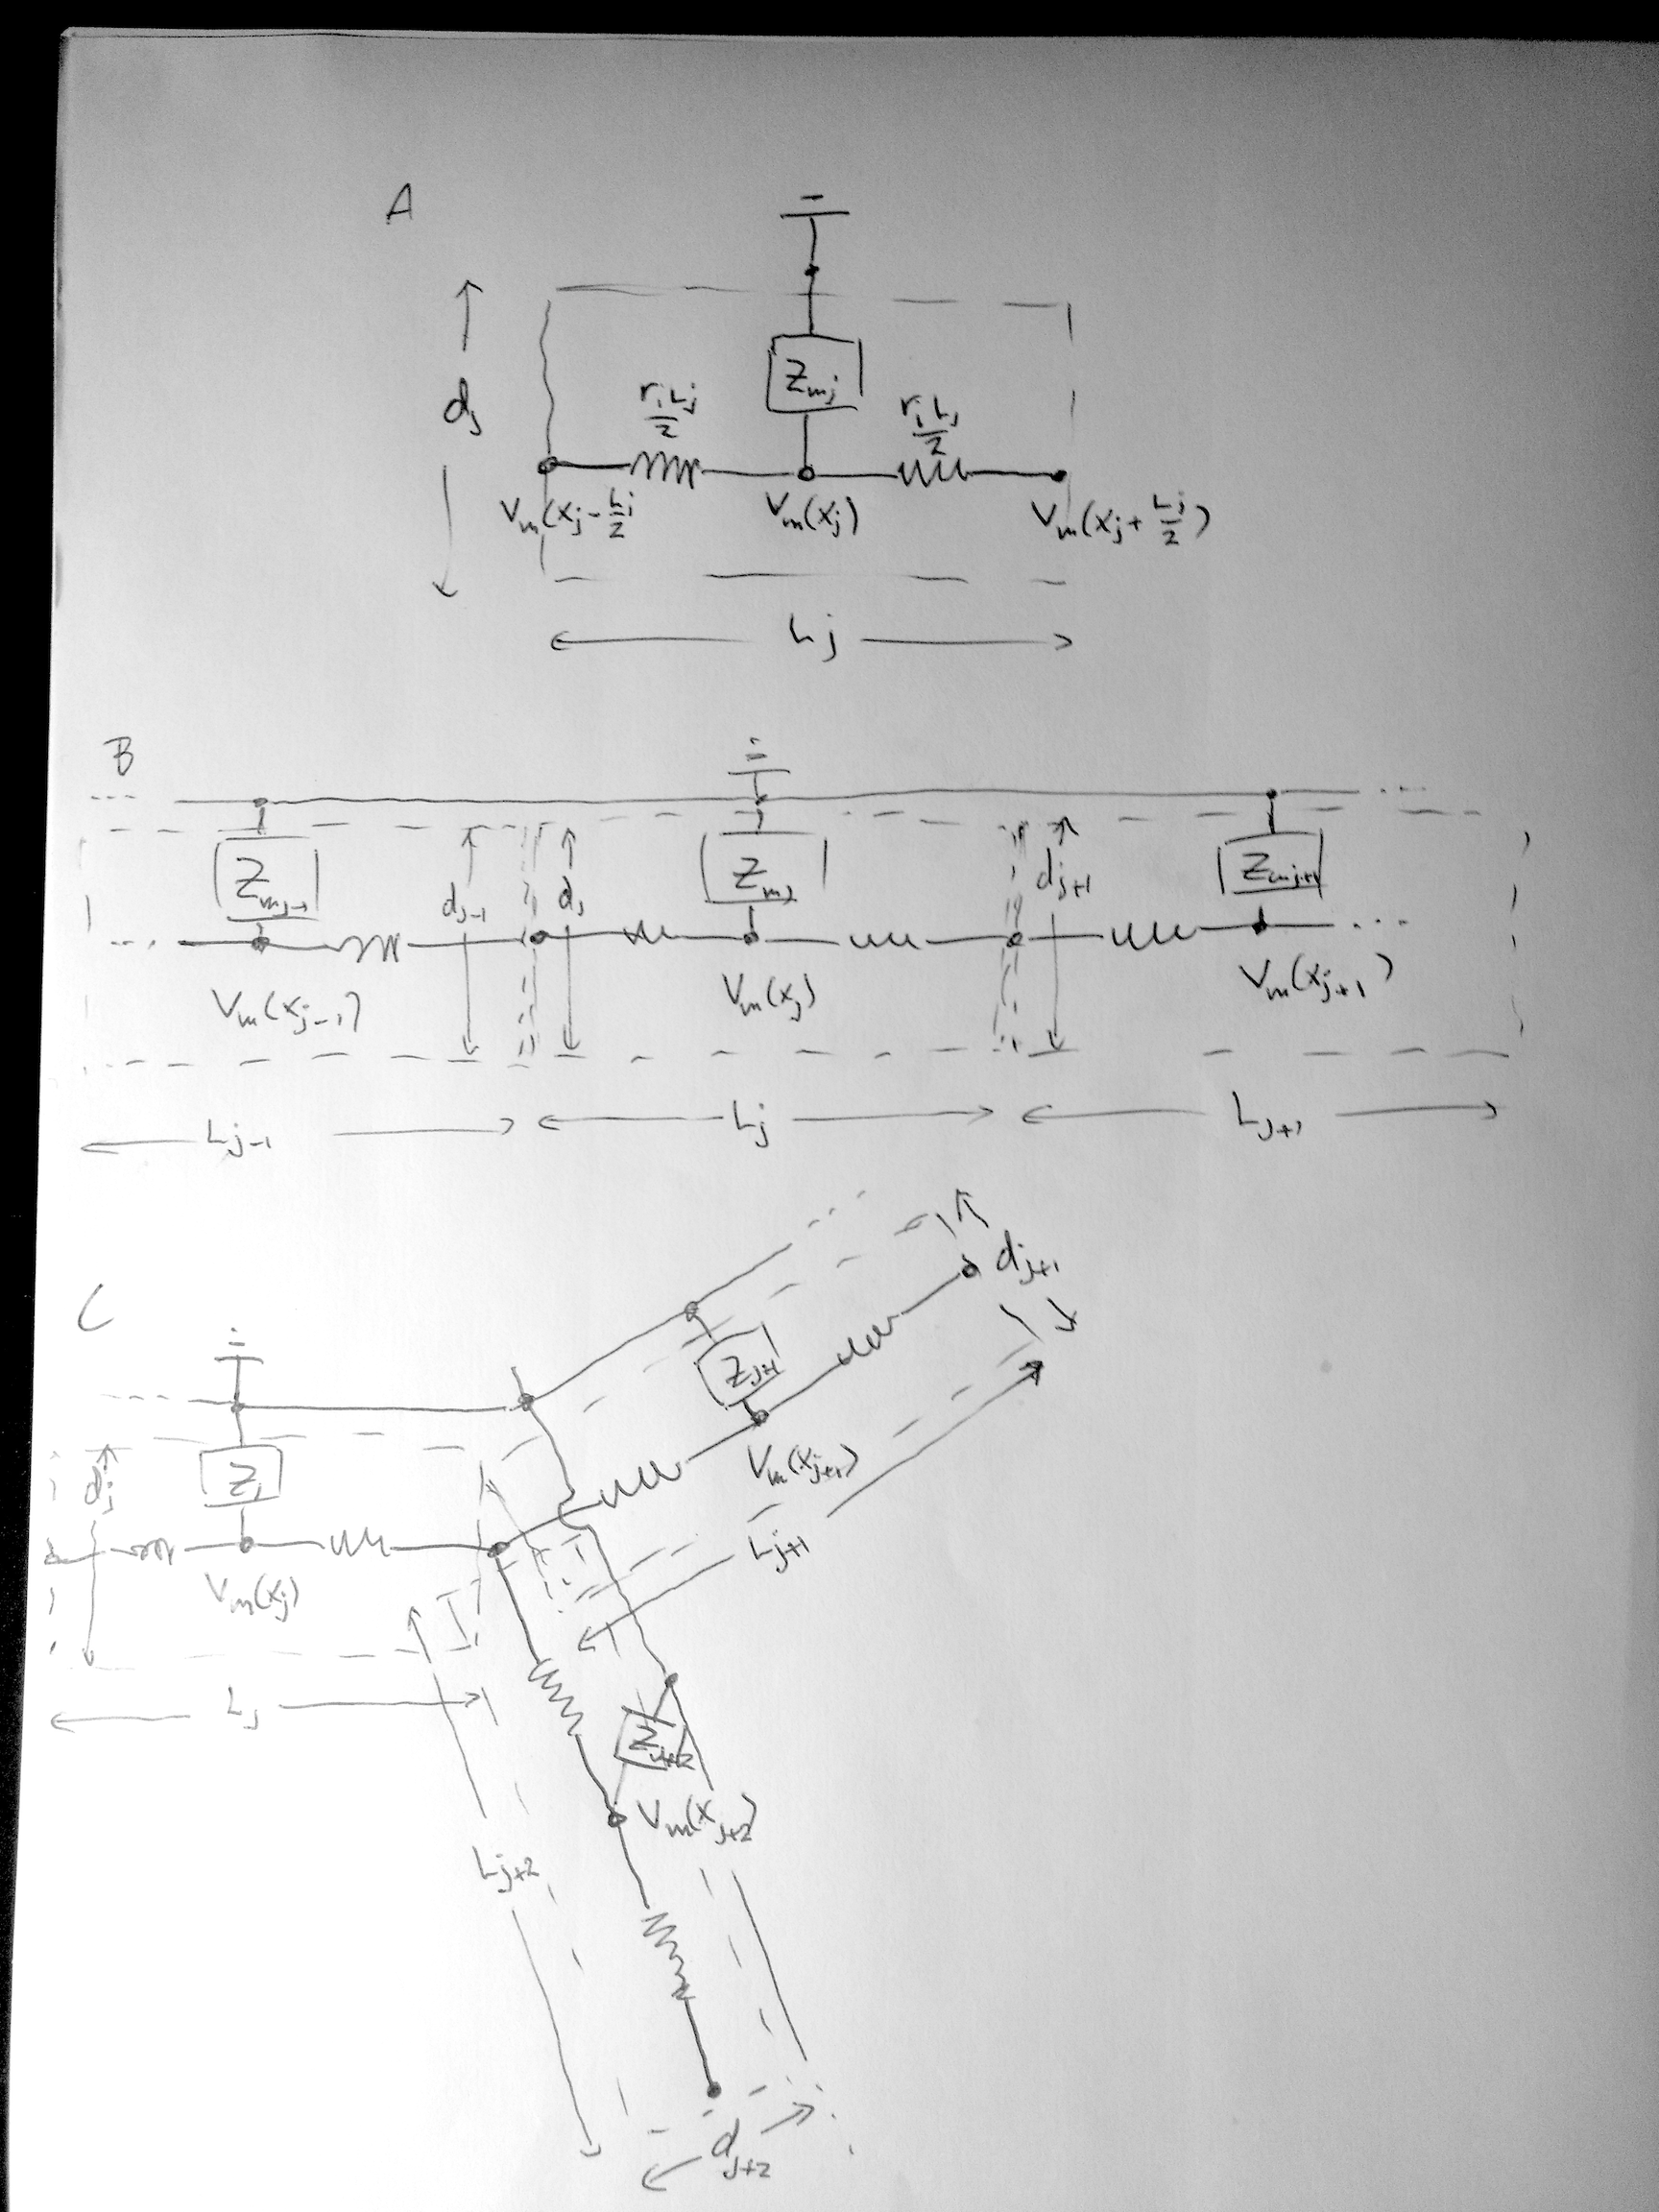
\includegraphics[width=0.8\textwidth]{Figures/Ch-LFPy/circuits.png}
\end{center}
\caption{\textbf{Equivalent circuits for computing axial and transmembrane currents}.
({\bf A}) One-compartment cable model with sealed ends.
({\bf B}) Continuous piece of MC cable model.
({\bf C}) MC cable model with branch point.}
\label{fig:LFPy_circuits}
\end{figure}


Up to this point, the attentive reader of this chapter may have noticed that the axial currents (and transmembrane currents for that matter) is \textit{linearly} dependent on the midpoint membrane voltages of the MC model.
Thus, the full set of operations involved in computing the full set of axial current magnitudes can be rewritten as a linear combination on the form
%
\begin{eqnarray}
\begin{bmatrix}
I_\mathrm{a}(\mathbf{r}_1, t)\\
I_\mathrm{a}(\mathbf{r}_2, t)\\
\vdots \\
I_\mathrm{a}(\mathbf{r}_N, t)
\end{bmatrix}
&=& \mathbf{A}^{-1}
\begin{bmatrix}
V_\mathrm{m}(\mathbf{r}_1, t)\\
V_\mathrm{m}(\mathbf{r}_2, t)\\
\vdots \\
V_\mathrm{m}(\mathbf{r}_N, t)\\
\end{bmatrix} ~,
\label{eq:LFPy_linear_combination}
\end{eqnarray}
%
where $\mathbf{r}_j$ denotes the midpoint location of compartment $j$ while the elements of the shape $(N, N)$ matrix $\mathbf{A}$ effectively corresponds to intracellular resistances and the specific connectivity between compartments
(recall Ohm's law for the current $I$ across a resistor $R$ given a voltage difference $\Delta V$: $I=R^{-1} \Delta V$).
$\mathbf{A}$ may in practise be non-invertible,
but it can be demonstrated that a matrix $\mathbf{G}\equiv \mathbf{A}^{-1}$ can be computed directly.
%
For a two-compartment model connecting the end point of the root (parent) compartment with the start point of the child compartment,
it can be shown with some arithmetics that the axial current in each compartment is \ehnote{derived in /sympycodes/Ch6\_calc\_iaxial.ipynb}
%
\begin{equation}
I_\mathrm{a}(\mathbf{r}_1, t) = I_\mathrm{a}(\mathbf{r}_2, t) =
	- \frac{\pi d_{1}^{2} d_{2}^{2} \left(V_\mathrm{m}(\mathbf{r}_1, t) - V_\mathrm{m}(\mathbf{r}_2, t) \right)}{4 R_{a} \left(L_{1} d_{2}^{2} + L_{2} d_{1}^{2}\right)} ~,
\end{equation}
%
which can be rewritten as the linear combination
%
\begin{eqnarray}
\begin{bmatrix}
I_\mathrm{a}(\mathbf{r}_1, t)\\
I_\mathrm{a}(\mathbf{r}_2, t)
\end{bmatrix}
=
- \frac{\pi d_{1}^{2} d_{2}^{2}}{4 R_{a} \left(L_{1} d_{2}^{2} + L_{2} d_{1}^{2}\right)}
\begin{bmatrix}
1 & -1 \\
1 & -1
\end{bmatrix}
\begin{bmatrix}
V_\mathrm{m}(\mathbf{r}_1, t) \\
V_\mathrm{m}(\mathbf{r}_2, t)
\end{bmatrix} ~,
\end{eqnarray}
%
that is, similar to \Fref{eq:LFPy_linear_combination}.
We encourage the interested reader of this book to show that the same approach hold for other model configurations, such
as 3-compartment models without and with branching points as illustrated in \Fref{fig:LFPy_circuits}B and C.

So far the axial currents is represented as a scalar field.
For some applications, such as computing the magnetic field $\mathbf{H}(\mathbf{r}, t)$,
the axial currents can be represented as a vector field by multiplication with the path vectors along the center axis of each compartment:
%
\begin{equation}
\mathcal{I}_\mathrm{a}(t) \equiv
\begin{bmatrix}
\mathbf{I}_\mathrm{a}(\mathbf{r}_1, t)\\
\mathbf{I}_\mathrm{a}(\mathbf{r}_2, t)\\
\vdots \\
\mathbf{I}_\mathrm{a}(\mathbf{r}_N, t)
\end{bmatrix}
=
\begin{bmatrix}
I_\mathrm{a}(\mathbf{r}_1, t) \mathbf{d}_1 \\
I_\mathrm{a}(\mathbf{r}_2, t) \mathbf{d}_2 \\
\vdots \\
I_\mathrm{a}(\mathbf{r}_N, t) \mathbf{d}_N
\end{bmatrix} ~,
\end{equation}
%
For compactness we introduced the current displacement $\mathbf{d}_j=\mathbf{r}_{\mathrm{f}j} - \mathbf{r}_{\mathrm{i}j}$,
where $\mathbf{r}_{\mathrm{i}j}$ and $\mathbf{r}_{\mathrm{f}j}$ denotes the start and end point coordinates of compartment $j$.
Consistent with the point-source formalism (cf. \Fref{sec:VC:pointsource}),
we let the `location' of each axial current be the mid-point $\mathbf{r}_j$ of each cylindrical compartment $j$.
In a similar manner we will represent the total transmembrane current per compartment as a matrix
\begin{equation}
\mathbf{I}_\mathrm{m}(t) =
\begin{bmatrix}
I_\mathrm{m}(\mathbf{r}_1, t) \\
I_\mathrm{m}(\mathbf{r}_2, t) \\
\vdots \\
I_\mathrm{m}(\mathbf{r}_N, t)
\end{bmatrix}
=
\begin{bmatrix}
i_\mathrm{m}(\mathbf{r}_1, t) \Vert \mathbf{d}_1 \Vert \\
i_\mathrm{m}(\mathbf{r}_2, t) \Vert \mathbf{d}_2 \Vert \\
\vdots \\
i_\mathrm{m}(\mathbf{r}_N, t) \Vert \mathbf{d}_N \Vert
\end{bmatrix} ~,
\end{equation}
under the assumption that the transmembrane current density $i_\mathrm{m}(x_j, t)$ is constant along the compartment axis.
Here, $\Vert\mathbf{d}_j \Vert$ denotes the norm of $\mathbf{d}_j$.
Note that $\mathcal{I}_\mathrm{a}(t)$ is a 3D tensor array with unit \si{\ampere \metre} and shape $(N, 3, N_t)$,
while $\mathbf{I}_\mathrm{m}(t)$ is a 2D matrix with unit \si{A} with shape $(N, N_t)$.
$N_t$ is here the number of discrete time steps in the simulated output signals.


%%%%%%%%%%%

\subsubsection{Application of linear volume conductor models for extracellular potentials and magnetic fields}

As derived from \textit{volume conductor theory} (\Fref{chap:VC}),
the different electric and magnetic signals that can be computed from the electric activity of brain cells are \textit{linearly} dependent on either transmembrane currents or axial currents.
Thus, some arbitrary signals $v(\mathbf{R}_i, t)$ in $M$ different spatial locations from the $N$ compartmental sources located at $r_j$ can be computed as
%
\begin{eqnarray}
\begin{bmatrix}
v(\mathbf{R}_1, t) \\
v(\mathbf{R}_2, t) \\
\vdots \\
v(\mathbf{R}_M, t)
\end{bmatrix}
&=& \mathbf{F}
\begin{bmatrix}
w(\mathbf{r}_1, t) \\
w(\mathbf{r}_2, t) \\
\vdots \\
w(\mathbf{r}_N, t)
\end{bmatrix} ~,
\end{eqnarray}
%
where $\mathbf{F}$ is a matrix with dimensions $(M, N)$ wherein each element $f_{ij}$ is the chosen forward solution mapping the contribution from each source to the corresponding measurement.
For the sake of compactness, $w(\mathbf{r}_j, t)$ is here either represents the axial or transmembrane current of compartment $j$. 
A simple linear forward model mapping transmembrane currents of an $N$-compartment model to extracellular potentials in $M$ locations would be the point-source formalism,
which models neuronal sources \textit{and} measurement sites as infinitesimally small points an infinite homogeneous isotropic and linear volume conductor.
The point-source formula (\Fref{eq:VC:pointsource}) results in
%
\begin{equation}
f_{ij} = \frac{1}{4\pi\sigma_\mathrm{e}}\frac{1}{\Vert\mathbf{R}_i - \mathbf{r}_j\Vert}  ~.
\end{equation}
%
The full linear system for obtaining the extracellular potential may then be written out as the linear combination
%
\begin{equation}
\begin{bmatrix}
\phi(\mathbf{R}_1, t) \\
\phi(\mathbf{R}_2, t) \\
\vdots \\
\phi(\mathbf{R}_M, t)
\end{bmatrix}
= \frac{1}{4\pi\sigma_\mathrm{e}}
\begin{bmatrix}
\frac{1}{\Vert\mathbf{R}_1 - \mathbf{r}_1\Vert} & \frac{1}{\Vert\mathbf{R}_1 - \mathbf{r}_2\Vert} & \cdots & \frac{1}{\Vert\mathbf{R}_1 - \mathbf{r}_N\Vert} \\
\frac{1}{\Vert\mathbf{R}_2 - \mathbf{r}_1\Vert} & \frac{1}{\Vert\mathbf{R}_2 - \mathbf{r}_2\Vert} & \cdots & \frac{1}{\Vert\mathbf{R}_2 - \mathbf{r}_N\Vert} \\
\vdots & \vdots & \cdots & \vdots \\
\frac{1}{\Vert\mathbf{R}_M - \mathbf{r}_1\Vert} & \frac{1}{\Vert\mathbf{R}_M - \mathbf{r}_2\Vert} & \cdots & \frac{1}{\Vert\mathbf{R}_M - \mathbf{r}_N\Vert}
\end{bmatrix}
\begin{bmatrix}
I_\mathrm{m}(\mathbf{r}_1, t) \\
I_\mathrm{m}(\mathbf{r}_2, t) \\
\vdots \\
I_\mathrm{m}(\mathbf{r}_N, t)
\end{bmatrix} ~.
\end{equation}
%
Note that the constant terms have been moved out of the matrix multiplication.
Similarly, for line sources (\Fref{eq:VC:linesource}), the elements of $\mathbf{F}$ may be calculated as
%
\begin{equation}
f_{ij} = \frac{1}{4\pi \sigma_\mathrm{e} \Delta s_{ij}} \log \left| \frac{\sqrt{h_{ij}^2+\rho_{ij}^2}-h_{ij}}{\sqrt{\ell_i^2+\rho_{ij}^2}-\ell_{ij}} \right| ~,
\label{eq:LFPy:linesources}
\end{equation}
%
where $\rho_{ij}$ is the distance perpendicular to line segment (compartment) $j$,
$h_{ij}$ the longitudinal distance from the end of the segment
and $\ell_{ij} = \delta s_{ij} + h_{ij}$ the longitudinal distance from the start of the segment to some electrode contact located at $\mathbf{R}_i$.

The approach is applicable also to other types of measurements which are linearly dependent on the transmembrane current sources,
such as the current dipole moment (\Fref{eq:VC:dipole}).
For computing the current dipole moment the mapping matrix' columns are simply
%
\begin{equation}
f_{j} = \mathbf{r}_j
=
\begin{bmatrix}
x_j \\
y_j \\
z_j
\end{bmatrix} ~.
\end{equation}
%
Another example is computing the \textit{ground truth} current source density (CSD) \cite**{Pettersen2008,Hagen2016,Hagen2017},
that is, assigning the contribution of different compartments' transmembrane current to $M$ different spatial domains $\Omega_i$ as
%
\begin{equation}
f_{ij} = \frac{\Delta s_{ij\in \Omega_i}}{\Delta s_{ij} V_{\Omega_i}} ~,
\label{eq:LFPy:gtCSD}
\end{equation}
%
where $(\Delta s_{ij\in \Omega_i} / \Delta s_{ij}) \in [0, 1]$ denotes the fraction of the length of the segment within the domain $\Omega_i$ and
$V_{\Omega_i}$ the volume of the spatial domain.
The geometry of each volume is in principle arbitrary,
however they are typically assumed to be cylindrical or cubic.
Cylindrical volumes can be useful for computing the ground truth CSD alongside a laminar probe \cite**{Pettersen2008,Hagen2016,Hagen2017},
while the latter could be used to compute the ground truth CSD across evenly distributed voxels distributed in the full 3D space occupied by the neuronal sources.

The formalism may also be adapted for higher-dimensional source elements, that is,
the set of axial currents $\mathcal{I}_\mathrm{a}$ which in the present context can be represented by a 3D tensor arrays with shape $(M, 3, N_t)$.
To compute the magnetic field outside the neuron arising from axial currents one can
either sum up the individual contributions using the relevant Biot-Savart law \cite**{Blagoev2007,Hagen2018} as
%
\begin{equation}
\mathbf{B}(\mathbf{R}_i, t) = \frac{\mu}{4\pi} \sum_{j=1}^M \frac{\mathbf{I}_\mathrm{a}(\mathbf{r}_j, t) \times (\mathbf{R}_i - \mathbf{r}_j) }{\Vert \mathbf{R}_i - \mathbf{r}_j \Vert^3} ~,
\label{eq:LFPy_biotsavart1}
\end{equation}
%
where the magnetic permeability $\mu \approx \mu_0=4\pi\times 10^7$~\si{\henry/\metre} that is, approximately equal to the permeability in vacuum.
Alternatively,
one can build up a forward model matrix $\mathbf{F}$ element by element as
%
\begin{equation}
f_{ij} = - \frac{1}{4\pi} \frac{I_3 \times (\mathbf{R}_i - \mathbf{r}_j) }{\Vert \mathbf{R}_i - \mathbf{r}_j \Vert^3} ~,
\label{eq:LFPy_biotsavart2}
\end{equation}
%
where $I_3$ is the shape $3 \times 3$ identity matrix,
thus the elements $f_{ij}$ are of shape $3 \times 3$ and $\mathbf{F}$ will be of shape (N, M, 3, 3).
Assuming that each compartmental axial current $\mathbf{I}_\mathrm{a}(\mathbf{r}_j, t)$ is represented as a $3 \times N_t$ matrix,
the calculation of the magnetic field $\mathbf{B}$ in location $\mathbf{R}_i$ from all contributions is
%
\begin{equation}
\mathbf{B}(\mathbf{R}_i, t) = \sum_{j=1}^M f_{ij} \cdot \mathbf{I}_\mathrm{a}(\mathbf{r}_j, t) ~.
\label{eq:LFPy_biotsavart3}
\end{equation}
%
Note that application of \Fref{eq:LFPy_biotsavart1} or \Fref{eq:LFPy_biotsavart3} is interchangeable and context dependent.
In situations where axial currents ($I_\mathrm{a}(\mathbf{r}_j, t)$),
current displacement ($\mathbf{d}_j$) and locations ($\mathbf{r}_j$) can be stored separately it may make sense to precompute the full $\mathbf{F}$-matrix for all $N$ measurement sites at once which may demand a lot of system memory.

\ehnote{usikker paa hvor detaljert jeg skal gaa inn her. Python/numpy lar en gjoere en gjoere denne operasjonen for alle maaleposisjoner kompakt som}
\ehtxt{\url{B=(F @ I).sum(axis=1); B.shape=(N,3,Nt); F.shape=(N,M,3,3); I.shape=(M,3,Nt)}}
\ehnote{ogsaa usikker paa notasjon for matriseprodukt med nD matriser som her.}


\ehnote{add some on combining current dipole moment to distal measures of activity (EEG, MEG)}
For forward-model predictions of distal electric and magnetic measures of neural activity such as EEG and MEG recordings, 
some simplifying steps can be made. 
As these signals are measured at distances much greater than the typical extent of the neuronal sources, 
the discrete spatial distribution of transmembrane currents $\mathbf{I}_\mathrm{m}(t)$ may be 
treated as an equivalent current dipole moment (\Fref{sec:VC:dipole}) defined as the product
\begin{equation}
\mathbf{P}(t) = 
\begin{bmatrix}
\mathbf{r}_1 \\
\mathbf{r}_2 \\
\vdots \\
\mathbf{r}_N
\end{bmatrix}
\begin{bmatrix}
I_\mathrm{m}(\mathbf{r}_1, t) \\
I_\mathrm{m}(\mathbf{r}_2, t) \\
\vdots \\
I_\mathrm{m}(\mathbf{r}_N, t)
\end{bmatrix} ~, 
\end{equation}
which is equivalent to \Fref{eq:VC:dipole}. 
As $\mathbf{r}_j \equiv [x_j, y_j, z_j]^\top$ (the shape of the current dipole moment array will be $(3, n_t)$. 

In the relatively simple case of an infinite homogeneous volume conductor the extracellular potential resulting from the current dipole moment is
\begin{equation}
\phi(\mathbf{R}, t) = \frac{\mathbf{P}(t) \cdot (\mathbf{R-r})}{4 \pi \sigma \Vert \mathbf{R-r} \Vert^3} ~,
\label{eq:LFPy:dipolepotential}
\end{equation}
where $\mathbf{R}$ denotes the measurement site and $\mathbf{r}$ the assumed dipole location. 
For the sake of computing EEG surface potentials however, 
an infinite homogeneous volume conductor model is arguably a quite poor approximation to the different tissues of the head.  
As discussed in more detail throughout \Fref{chap:EEG} different forward models for EEG-like potentials has been developed in the past, 
either relying on representing different tissues as a series of concentric shells with different conductivities for each main tissue (gray matter, cerebral spinal fluid, skull etc.) \cite**{Nunez2006,Naess2017,Naess2020}, 
or even more detailed head models based on anatomical reconstruction such as the New York Head model \cite**{Huang2016}. 
Without going into any mathematical detail here (more on that in \Fref{chap:EEG}), 
these models generally can be written on the form of a linear combination
\begin{equation}
\phi(\mathbf{R, r}) = \mathbf{M}\mathbf{P}
\end{equation}
where the coefficients of the matrix $\mathbf{M}\equiv \mathbf{M}(\mathbf{R, r})$ is model dependent. 
From the current dipole moment potential (\Fref{eq:LFPy:dipolepotential}), 
the corresponding rows of $\mathbf{M}$ for each electrode site $\mathbf{R}_i$ can be computed as 
\begin{equation}
m_{i} = \frac{I_3 \cdot (\mathbf{R}_i-\mathbf{r})}{4 \pi \sigma \Vert \mathbf{R}_i-\mathbf{r} \Vert^3}~,
\end{equation}
where $I_3$ is the shape $3 \times 3$ identity matrix as above.
The resulting shape of $\mathbf{M}$ is $M \times 3$. 

As the extracellular potential remains linearly dependent on the current dipole moment $\mathbf{P}$ 
which in turn is linearly dependent on the transmembrane currents, 
one can with relative ease estimate a linear predictor of extracellular potentials from transmembrane currents via the current dipole moment by computing the matrices $\mathbf{M}$ and $\mathbf{F}$ and then estimate the final signal as 
\begin{equation}
\phi(\mathbf{R}, t) = \mathbf{M}\mathbf{F}\mathbf{I}_\mathrm{m}(t)~.
\end{equation}

\ehnote{show code examples from LFPykit?}




\section{\red{EH: Forward-model predictions from point-neuron models}}
\label{sec:Schemes:HybridLFPy}
\index{Point neuron model}

%\ehnote{gammalt:}
%%\sout{Point neuron models do not generate extracellular fields. Sad, because simulations would be much faster if we could use point neuron models. Trick to do this, Hybrid LFPy \cite**{Hagen2016}, Skaar et al (in revision)}

\ehnote{nytt:}
Many biophysically detailed and phenomenological models of individual neurons and neuronal networks that have been developed in the past have incorporated spatial geometry of the neurons at various level of detail. 
To represent and simulate the dynamics of such neuron models using computers the multicompartment cable formalism (\Fref{chap:Neuron}) remains a common choice. 
For the purpose of predicting extracellular electric or magnetic measures of neural activity, 
the multicompartment formalism (or variants thereof) is \emph{a priori} required in order to predict the spatial distribution of transmembrane or axial currents required for the different forward models derived using volume conductor theory (\Fref{chap:VC}). 

Biophysically detailed multicompartment neuron models (and recurrently connected networks thereof) are however computationally costly due to the large number of associated state variables that must be predicted, 
resulting in long simulation times on typical hardware. 
For recurrent neuronal network simulations with more than a few hundred biophysically detailed neurons, distributed high-performance computing (HPC) facilities are generally required, 
unless the neuronal simulation software may utilize some other form of hardware acceleration as facilitated by desktop graphical processing units (GPUs) for instance.  

As the most common observables used to experimentally assess evoked and ongoing neuronal activity have historically been timings of somatic action potentials (`spikes' - see \Fref{chap:Spikes}) and/or voltage traces, 
many (if not most) studies aiming to explain neuronal population dynamics at the level of spikes and somatic voltages have deliberately chosen much-simpler mathematical abstractions of the individual neurons. 
As an umbrella term such simple neuron models are often referred to as `point' neuron models if they can be considered as a singular compartment,
that is, 
the neuron model has no description of how the membrane potential vary throughout the dendrites and axon which may be present in actual neurons. 
Point neuron models as a consequence also then carries no spatial information about neuronal geometry.
The individual point neurons (or \emph{point processes}) may however be assigned locations corresponding to brain area, cortical layer, feature space (e.g., desired orientation tuning) or similar, 
which may facilitate connection routines that depend on location and distance between the neurons. 

Many point-neuron models describe at a minimum the sub-threshold membrane potential and may include some form of additional non-linearity representing times of emitted spikes and corresponding periods of refractoriness such as the leaky integrate-and-fire neuron model \cite**{Lapicque1907,Brunel_2007}.
We will here point out that describing the somatic voltage is not a strict requirement for point neurons in the present context - they may very well be some statistical model for spike time generation as function of presynaptic activity or some other stimuli. 

Their mathematical simplicity lends point neurons to be implemented and solved very efficiently in comparison to biophysically detailed multicompartment neuron models. 
As a consequence, dynamics of recurrently connected networks of spiking point neurons can be studied at a much grander scale and pace than similarly sized networks of multicompartment neuron models. 
As typical point neurons also have very few intrinsic parameters compared to any multicompartment neuron model, 
this has also allowed for separating effects of network connectivity from the cellular dynamics 
explaining observed phenomena such as asynchronous or synchronous, regular and irregular spiking activity also using rigorous mathematical analysis, see e.g., \cite**{Brunel2000}). 

Linking activity of point neurons and point neuron network models to electric or magnetic extracellular measures of activity however poses a problem. 
One could attempt to extract equivalent transmembrane currents (synaptic, ionic, capacitive etc.) and quickly come to the conclusion that all currents \emph{must} sum to zero in the point(s) due to charge conservation. 
As such there can be no electric or magnetic signals arising from point neurons or networks thereof. 
Physics-based computational schemes for predicting signals such as the local field potential (LFP) is therefore required. 

\subsection{The hybrid scheme}
\label{chap:LFPy:hybrid}

As constraining activity in large scale multicompartment neuron network models are inherently difficult due to the large number of parameters and huge computational demands, 
point neurons (or other simplified neuron representations) are more-often used in simulation studies of network activity. 
But for forward-model predictions, 
at least a two-compartment neuron model is \textit{a priori} required for it to account for spatial variations of in- and outgoing transmembrane currents giving rise to extracellular potentials or magnetic fields. 

One solution to this problem of deriving physics based schemes for computing extracellular electric or magnetic signals from point neuron networks was introduced by 
\cite**{Hagen2016}, 
referred to as a hybrid scheme. 
The scheme is hybrid in the sense that the common-place scheme of using multi-compartment neuron models in conjunction with electrostatic forward models is used for signal prediction, 
while it assumes that simulations of the actual network activity can be done independently using neuron models with arbitrary levels of detail, including point processes (LIF neurons etc.). 
In a latter step, 
generated spike times are used for activation times of synapses distributed onto multicompartment neuron models which allows using the standard computational scheme for predicting extracellular signals. 
We will next go through the number of assumptions and methodology underlying this scheme in detail. 

\begin{figure}[htbp]
\begin{center}
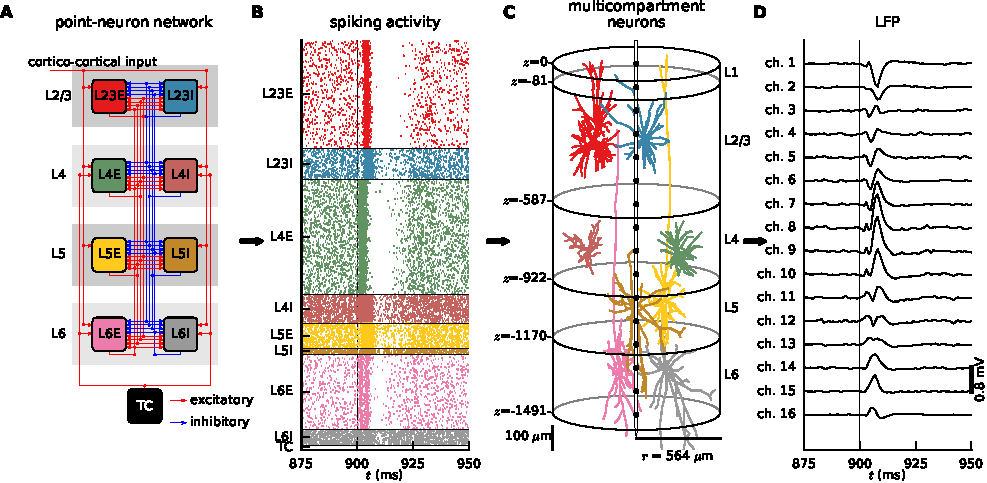
\includegraphics[width=\columnwidth]{Figures/Ch-LFPy/hybridmodel}
\caption{\ehnote{Hagen 2016 caption:} 
Overview of the hybrid LFP modeling scheme for a cortical microcircuit model. 
(A) Sketch of the point-neuron network representing a 
\SI{1}{\milli\metre} patch of early sensory cortex (adapted from Potjans2014). 
The network consists of 8 populations of LIF neurons, representing excitatory (E) and inhibitory neurons (I) in cortical layers 2/3, 4, 5, and 6. 
External input is provided by a population of TC neurons and cortico-cortical afferents. 
The color coding of neuron populations is used consistently throughout this paper. 
Red arrows: excitatory connections. Blue arrows: inhibitory connections. 
See Tables 1-2, 5-6 for details on the network model. 
(B) Spontaneous (t < \SI{900}{\milli\second}) and stimulus-evoked spiking activity (synchronous firing of TC neurons at time $t = $\SI{900}{\milli\second}, denoted by thin vertical line) generated by the point-neuron network model shown in panel A, sampled from all neurons in each population. Each dot represents the spike time of a particular neuron. 
(C) Populations of LFP-generating multicompartment model neurons with reconstructed, layer- and cell-type specific morphologies. 
Cells are distributed within a cylinder spanning the cortex. Layer boundaries are marked by horizontal black lines (at depths $z$ relative to cortex surface $z = 0$). Only one representative neuron for each population is shown 
(see Fig. 4 for a detailed overview of cell types and morphologies). 
Sketch of a laminar recording electrode (gray) with 16 contacts separated by \SI{100}{\micro\metre} (black dots). 
(D) Depth-resolved LFP traces predicted by the model (cf. Tables 3 and 4). 
Note that channel 1 is at the pial surface, so that channel 2 corresponds to a cortical depth of \SI{100}{\micro\metre} and so forth.
}
\label{fig:LFPy:hybridmodel}
\end{center}
\end{figure}



One main assumption is that point-neuron network models can accurately capture observations present in experimental data gathered \textit{in vivo}, 
including irregular firing patterns
\ehnote{(Softky and Koch 1993; van Vreeswijk and Sompolinsky 1996; Amit and Brunel 1997; Shadlen and Newsome 1998), membrane-potential fluctuations (Destexhe and Pare 1999), asynchronous firing (Ecker et al. 2010; Renart et al. 2010; Ostojic 2014), correlations in neural activity (Gentet et al. 2010; Okun and Lampl 2008; Helias et al. 2013), self-sustained activity (Ohbayashi et al. 2003; Kriener et al. 2014), and realistic firing rates across laminar cortical populations (Potjans and Diesmann 2014).}
Similarly, reduced models derived from biophysically detailed multicompartment neuron models has shown that point-neuron network models can accurately capture spiking statistics of the original model (see e.g., \cite**{Roessert2016,Billeh_2020}). 
In the case of \cite**{Roessert2016} the effect of dendritic filtering on synaptic input currents is captured by computing an equivalent filter for each possible synapse location and type using a Green's function formalism \cite**{Wybo_2013}. 
The point neurons are modeled using a generalized integrate-and-fire (GIF) formalism, 
and the linear filters applied to the synaptic currents result in  well-preserved post-synaptic potentials in the point neuron. \ehnote{perhaps I'll leave this last point out.}  

Another main assumption underlying the hybrid scheme is that spatial information, that is, neuronal geometry and locations of synapses can be `restored' \ehnote{noen bedre ord?} for the purpose of computing extracellular signals, 
based on available anatomical knowledge. 
This assumption entails that a point-neuron network population representing for instance a set of layer 5 pyramidal cells, 
will be represented by a corresponding population of geometrically detailed multicompartment neuron models, 
placed at a cortical depth and density in accordance with the overall network size and available anatomical constraints. 
Similarly, incoming synaptic connections onto the same point-neuron population from each presynaptic population, 
for instance layer 4 inhibitory interneurons, 
should be positioned onto the layer 5 pyramidal cell geometries according to rules derived from available data on such connections, 
while also preserving the typical number of incoming synapses (aka synaptic in-degree). 

In the original application of the hybrid scheme \cite**{Hagen2016} to a point-neuron network model representing a generic cortical microcircuit \cite**{Potjans2014}, 
a number of parameters of the network model were inherited by the  forward-modeling step. 
In order to preserve synaptic currents, 
the same current-based synapse type (see \Fref{sec:Ch-Neuron:current-based-syn}) with an exponentially decaying temporal kernel were used, 
with the same average maximum current amplitude, 
and with activation delays drawn from the same conduction delay distribution as was used in the network. 
Synapse sites on the postsynaptic morphologies were derived from a connectivity dataset resolving numbers of synapses per layer between 16 different excitatory and inhibitory neuron types spanning layers 2/3, 4, 5 and 6.
The total numbers of synapses per connection (from each presynaptic to postsynaptic population) were preserved. 
Furthermore, membrane time constants of the reconstructed morphologies which utilized purely passive compartments throughout were set similar to those of the point neurons. 
\ehnote{kunne lagt til noe om ekspandering av enkelte punktnevronpopulasjoner til forskjellige celletyper som vi gjorde den gang.} 

One key feature of the this hybrid scheme application as devised by \cite**{Hagen2016} was an assumed-to-be \emph{linear} spike-LFP relationship, 
that is, 
one spike generated by a network subpopulation would result in a fixed contribution to the extracellular signal resulting from synaptic and transmembrane currents on postsynaptic multicompartment neurons.  
So how can we make an argument about the validity of said scheme, 
e.g., in the presence of \emph{non-linear} synaptic and ion-specific channels?
Conceptually, it is perhaps best to first consider a recurrently connected network of biophysically detailed neurons, 
and that the aforementioned point-neuron network model represents something of an idealized scenario obtained by reducing biophysical detail in a systematic manner.

Let us first define some properties of the biophysically detailed model:
\begin{enumerate}
\item Let $X \in \{ \ldots \}$ and $Y \subseteq X$ denote pre- and postsynaptic population, respectively. Each population corresponds to separate classes of neurons (derived from anatomy, electrical properties, gene expression etc.).
\item Let $N_X$ and $N_Y$ denote the sizes of population $X$ and $Ys$.
\item Let $i \in \{ 1, \ldots , N_X \}$ and $j \in \{ 1, \ldots , N_Y \}$ denote pre- and postsynaptic neuron index, respectively.
\item Let $\mathbf{r}_i \in \Omega_X$ denote the discrete somatic location of neuron $i$ in a volumetric domain $\Omega_X$
\item Let $K_{YX}$ denote the total number of synapses between presynaptic population $X$ and postsynaptic population $Y$. 
Assuming a random connectivity with binomial in- and out-degree distributions the corresponding connection probability is then $C_{YX}=1-(1-1/{N_Y N_X})^{K_{YX}}$ \cite**{Potjans2014}. 
\item Let layer or region (e.g., cortical layer) be denoted by $L$.
\item Let synapse placement be described by a spatial probability function $\mathcal{L}_{YXL} \geq 0 $ such that $\sum_L \mathcal{L}_{YXL} := 1$ if $K_{YX} > 0$ and 0 if $K_{YX} = 0$.
\item Synaptic currents for each connection are given as $i_{\mathrm{syn}YX}(t)=\overline{g}_{\mathrm{syn}YX} f(t)(V(t)-E_{\mathrm{syn}Y}$
where $\overline{g}_{\mathrm{syn}YX}$ is the maximum synaptic conductance and $f(t) \in [0, 1]$ is one of the temporal kernels listed in \Fref{sec:Ch-Neuron:conductance-based-synapses}. 
$V(t)$ denotes the postsynaptic potential and $E_{\mathrm{syn}Y}$ denotes the reversal potential of the synapse which is determined by the presynaptic cell type (i.e., excitatory or inhibitory). 
For simplicity we will assume that conductance magnitude is independent of $L$. 
\item The conduction delay from presynaptic action potential generation time  to activation time of the synapse $d_{YX}$ be constant (i.e., independent of cell location and geometry for simplicity). 
\item Each postsynaptic neuron $j \in Y$ is modeled using the  `standard' multicompartment neuron formalism such that their transmembrane currents $\mathbf{I}_\mathrm{m}^{\langle j \rangle}(t)$ or axial currents $\mathcal{I}_\mathrm{a}^{\langle j \rangle}(t)$ can be computed. 
Here $X$ and $Y$ may be used interchangeable, however, 
presynaptic populations may represent point processes, external stimuli and similar, which we will assume give approximately zero direct contributions to the signals predicted by the full network model.
\item Extracellular signal contributions in different spatial locations may be computed and summed up as 
$\sum_Y \sum_{j=1}^{N_Y} \mathbf{F}^{\langle j \rangle} \mathbf{I}_\mathrm{m}^{\langle j \rangle}$ and similar for axial currents. 
$\mathbf{F}^{\langle j \rangle}$ here denotes a linear mapping of transmembrane currents of cell $j$ to a linearly dependent signal.  
\item The set of spike times $\{ t_\mathrm{s}^{\langle i \rangle} \}$ of each of each neuron $i \in X$ is recorded throughout the entire simulation interval $[0, T_\mathrm{sim} \rangle$. 
We may choose to relax this requirement if a population $X$ represents an external population feeding persistent, uncorrelated events with `flat' spiking statistics (e.g., Poisson point process) into the recurrently connected network. 
\item We may store the directed graph representing vertices (connections) between nodes (neurons) for every pair of pre- and postsynaptic population. 
This requirement may also be relaxed if the total number of connections $K = \sum_X \sum_Y K_{YX}$ is large enough to make storage infeasible or one could recreate the full graph from the model specification (at least statistically). 
\end{enumerate}





\section{\red{EH: Neurodynamics using firing-rate models}}
\label{sec:Schemes:KernelLFPy}
\index{Firing rate model}

\ehnote{gammalt:}
Would make things even faster. Population firing-rate models  \cite**{Hagen2016}. Kernel trick (Ness et al, on-going project)

\ehnote{nytt:}


%%%%%%%%%%%%%%%%%%%%%%%%%%%%%%%%%%%%%%%%%%%%%%%%%%%%%%%%%%%%%%%%

\section{\blue{GH: Self-consistent scheme for intra- and extracellular potentials} }
\label{sec:VC:EMI}
\index{Ephaptic effects}
Ephaptic effects refers to the phenomenon where the extracellular potential affects the membrane potential dynamics of neurons. The possible importance of ephaptic effects has been the topic of many studies, addressing in various ways how extracellular electric fields may affect neuronal firing or signal propagation in axons (see e.g., \cite**{clark1970,Rall1977,Holt1999,Bokil2001,anastassiou2010,anastassiou2015,Goldwyn2016,capllonch2020,ruffini2020}).

Most of these studies have been based on some simplified approximations as to how evoked fields from one neuron affects other neurons, and less focus has been put on how the presence of ephaptic effects will affect the extracellular potential itself. Rigorous modeling of this, requires that the intra- and extracellular dynamics are modeled simultaneously on a unified framework based on VC theory. Such a framework exists \cite**{Krassowska1994,Agudelo-Toro2013,Tveito 2017}, and was in a recent publication referred to as the extracellular-membrane-intracellular (EMI) framework \cite**{Tveito2017}.

We here only describe very briefly the essence of the EMI framework. It is based on (Ohmic) current conservation in the intra- and extracellular spaces, so that:
\begin{equation}
\nabla \cdot \sigma_r \nabla \phi_r = 0,
\label{eq:VC:EMI}
\end{equation}
where $r$ takes the indexes $i$ (intracellular space) or $e$ (extracellular space). The intra- and extracellular dynamics are coupled through suitable boundary condictions at the membrane, making sure that a current \textit{entering} the membrane (normal component) at one side of the membrane, is constrained to be identical to the current \textit{leaving} the membrane (negative normal component) on the opposite side \cite**{Krassowska1994}. These entering and leaving currents are in turn determined by a set of mechanisms that jointly determine the transmembrane current $I_m$. In previous numerical implementations of the EMI framework, the membrane currents were modeled with Hodgkin-Huxley like kinetics \cite**{Agudelo-Toro2013,Tveito2017}.

Compared to the two-step MC+VC framework, EMI has the disadvantage that it is computationally expensive. In the MC + VC scheme, which uses volume conduction modeling only for the extracellular space, $\phi_e$ can be computed as an analytical function of the transmembrane neural currents (cf. Chapter \ref{chap:VC}). Using EMI, analytical examples of solutions can only be obtained for idealized scenarios \cite**{Krassowska1994}, while general EMI applications require that both the intra- and extracellular spaces are spatially resolved and their dynamics computed on a numerical framework \cite**{Agudelo-Toro2013,Tveito2017}.

Using EMI to simulate larger systems with realistic morphologies would probably exceed the capacity of today's computers. However, EMI has been used to perform a systematic exploration of the inaccuracies induced when ignoring ephaptic effects in a small system of neurons represented with stylized geometries  \cite**{Tveito2017}.

There exist even more advanced framework than EMI, which, in addition to accounting for ephaptic effects, also account for effects of changing ion concentrations. We will talk briefly of this in Chapter \ref{sec:Eldiff}, where we consider electrodiffusive transports in brain tissue.
